This document collects notes about the HSC PDR1 reprocessing in cycle S18.
Background information can be found in the notes of S17B HSC PDR1 reprocessing (\url{https://confluence.lsstcorp.org/display/DM/S17B+HSC+PDR1+reprocessing}).
The nominal ticket for the S18 PDR1 run is \jira{DM-13666}.

The output repos are:

\begin{enumerate}
\item
/datasets/hsc/repo/rerun/DM-13666/UDEEP/
\item
/datasets/hsc/repo/rerun/DM-13666/DEEP/
\item
/datasets/hsc/repo/rerun/DM-13666/WIDE/
\end{enumerate}

\section{Input dataset}

HSC SSP PDR1 data, as described in \citeds{DMTR-31} Sect 1; this is the same as S17B HSC PDR1 reprocessing. It includes 5654 visits in 7 bands and 3 layers (386 visits in UDEEP, 668 visits in DEEP, and 4600 visits in WIDE). It has 11 tracts in UDEEP, 37 tracts in DEEP, and 91 tracts in WIDE.
The tract IDs can be found in \url{https://hsc-release.mtk.nao.ac.jp/doc/index.php/database/} (except tract=9572) or the first table on the S17B HSC PDR1 reprocessing page.

The calibration repo is version \texttt{20180117}, located at \texttt{/datasets/hsc/calib/20180117}  (from \jira{DM-13387})


\section{Software stack version}
The processing will use stack version \texttt{w\_2018\_15} (released 2018-04-16).

For verification, the RC2 reprocessing of \texttt{w\_2018\_14} is at \jira{DM-13890} and the RC2 reprocessing of \texttt{w\_2018\_15} is at \jira{DM-14123}.

Pipeline steps and execution units
\begin{enumerate}
\item
makeSkyMap.py:   One SkyMap for the whole campaign
\item
singleFrameDriver.py:   independent per ccd, typically run per visit
\item
skyCorrection.py:   per visit
\item
mosaic.py:   per tract x filter, including all visits overlapping that tract in that filter.
\item
coaddDriver.py: independent per patch, run per tract x filter, including all overlapping visits
\item
multiBandDriver.py:   independent per patch, may run per tract, including all filters
\end{enumerate}
Data of different layers (DEEP/UDEEP/WIDE) are processed separately.


\section{Pipeline configurations}
The HSC default config will be used. ccd=9 is not processed as it has bad amps and results not trustworthy even if processCcd passes.

Operational configurations can be different from the stack defaults; e.g. can make \texttt{config.assembleCoadd.subregionSize} small enough so a full stack of images can fit into memory at once; a trade-off between memory and i/o but doesn't matter scientifically, as the pixels are independent. Also, pipe\_drivers jobs can be continued with the \texttt{--reuse-outputs-from all} option, rather than starting over.


\section{Reproducible Failures}
In singleFrameDriver/processCcd, there were reproducible failures in 14 CCDs in the UDEEP layer, 6 CCDs in the DEEP layer, and 120 CCDs in the WIDE layer.  Their data IDs are:

UDEEP

\texttt{--id visit=17934 ccd=1 --id visit=19712 ccd=33 --id visit=23596 ccd=6 --id visit=37828 ccd=101 --id visit=38494 ccd=4 --id visit=38494 ccd=6 --id visit=38494 ccd=11 --id visit=38494 ccd=32 --id visit=38494 ccd=37 --id visit=38494 ccd=43 --id visit=38494 ccd=54 --id visit=38494 ccd=80 --id visit=38494 ccd=96 --id visit=38494 ccd=102}

DEEP

\texttt{--id visit=19702 ccd=12 --id visit=22640 ccd=10 --id visit=24342 ccd=102 --id visit=9664 ccd=94 --id visit=36842 ccd=94 --id visit=15206 ccd=100}

WIDE

\texttt{--id visit=6342 ccd=11 --id visit=6478 ccd=99 --id visit=6528 ccd=24 --id visit=6528 ccd=59 --id visit=6528 ccd=67 --id visit=6528 ccd=75 --id visit=6542 ccd=96 --id visit=7344 ccd=67 --id visit=7356 ccd=96 --id visit=7408 ccd=84 --id visit=9708 ccd=99 --id visit=9736 ccd=67 --id visit=9748 ccd=96 --id visit=9838 ccd=101 --id visit=9868 ccd=76 --id visit=11406 ccd=22 --id visit=11414 ccd=66 --id visit=11582 ccd=76 --id visit=11614 ccd=101 --id visit=11640 ccd=70 --id visit=13166 ccd=20 --id visit=13178 ccd=91 --id visit=13182 ccd=101 --id visit=13198 ccd=84 --id visit=13198 ccd=85 --id visit=13198 ccd=90 --id visit=13198 ccd=91 --id visit=13288 ccd=84 --id visit=15096 ccd=47 --id visit=15096 ccd=54 --id visit=16064 ccd=101 --id visit=17670 ccd=24 --id visit=17672 ccd=24 --id visit=17692 ccd=7 --id visit=17692 ccd=8 --id visit=17722 ccd=20 --id visit=17736 ccd=63 --id visit=17738 ccd=69 --id visit=17750 ccd=58 --id visit=19394 ccd=24 --id visit=19414 ccd=8 --id visit=19454 ccd=20 --id visit=19468 ccd=69 --id visit=19646 ccd=2 --id visit=25894 ccd=68 --id visit=25956 ccd=76 --id visit=25968 ccd=65 --id visit=26054 ccd=43 --id visit=27068 ccd=96 --id visit=29378 ccd=70 --id visit=29898 ccd=99 --id visit=29916 ccd=99 --id visit=29936 ccd=66 --id visit=29942 ccd=96 --id visit=29966 ccd=103 --id visit=30588 ccd=98 --id visit=31410 ccd=73 --id visit=32506 ccd=3 --id visit=32506 ccd=8 --id visit=33824 ccd=56 --id visit=33862 ccd=8 --id visit=33890 ccd=61 --id visit=33934 ccd=95 --id visit=33950 ccd=52 --id visit=33950 ccd=60 --id visit=34268 ccd=103 --id visit=34332 ccd=61 --id visit=34334 ccd=61 --id visit=34348 ccd=100 --id visit=34410 ccd=58 --id visit=34412 ccd=78 --id visit=34634 ccd=61 --id visit=34636 ccd=61 --id visit=34684 ccd=58 --id visit=34748 ccd=85 --id visit=34928 ccd=61 --id visit=34930 ccd=61 --id visit=34934 ccd=101 --id visit=34936 ccd=50 --id visit=34938 ccd=95 --id visit=35852 ccd=8 --id visit=35862 ccd=61 --id visit=35882 ccd=19 --id visit=35892 ccd=12 --id visit=35894 ccd=86 --id visit=35908 ccd=28 --id visit=35916 ccd=50 --id visit=35942 ccd=4 --id visit=35942 ccd=64 --id visit=35948 ccd=72 --id visit=35966 ccd=60 --id visit=36178 ccd=98 --id visit=36216 ccd=6 --id visit=36264 ccd=94 --id visit=36604 ccd=81 --id visit=37532 ccd=33 --id visit=37538 ccd=100 --id visit=37552 ccd=12 --id visit=37988 ccd=33 --id visit=38316 ccd=11 --id visit=38328 ccd=91 --id visit=38330 ccd=8 --id visit=38346 ccd=8 --id visit=38912 ccd=86 --id visit=42218 ccd=102 --id visit=42222 ccd=102 --id visit=42454 ccd=17 --id visit=42454 ccd=24 --id visit=42510 ccd=77 --id visit=42534 ccd=65 --id visit=44050 ccd=94 --id visit=44060 ccd=31 --id visit=44090 ccd=27 --id visit=44154 ccd=66 --id visit=44160 ccd=55 --id visit=44162 ccd=61 --id visit=45262 ccd=64 --id visit=45348 ccd=64 --id visit=45940 ccd=47 --id visit=46892 ccd=64}

Out of the 140 failures:

\begin{enumerate}
\item
58 failed with "Unable to match sources"
\item
31 failed with "No matches to use for photocal"
\item
12 failed with "No objects passed our cuts for consideration as psf stars"
\item
2 failed with "Unable to measure aperture correction for required algorithm 'modelfit\_CModel\_exp': only [01] sources, but require at least 2."
\item
37 failed with "InvalidParameterError: 'Only spatial variation (ndim == 2) is supported; saw 0'" which trace back to "PSF star selector found [123] candidates" in processCcd.charImage.measurePsf
\end{enumerate}

Rerun logs of these failures are attached in \jira{DM-13667}


In coaddDriver, there were no FATAL- or ERROR-level log records, but many WARN-level records.  Among them there were three kinds of "errors" in edge patches.

\jira{DM-14282} "cannot do a non-empty take from an empty axes" in 8 patches:

\texttt{(UDEEP) --id tract=8766 filter=HSC-G patch=8,3
(UDEEP) --id tract=9571 filter=HSC-Y patch=7,7
(DEEP) --id tract=9708 filter=HSC-G patch=7,6
(DEEP) --id tract=9812 filter=HSC-G patch=5,3
(DEEP) --id tract=8766 filter=HSC-I patch=0,5
(DEEP) --id tract=9707 filter=HSC-I patch=6,6
(DEEP) --id tract=9707 filter=NB0816 patch=6,6
(WIDE) --id tract=16972 filter=HSC-G patch=0,7
}

\jira{DM-14286} CompareWarpAssembleCoadd RuntimeError when No PsfMatched warps found at edge cases despite no psfMatchedWarp files were written because there were 0 good pixels, in 5 patches:

\texttt{(DEEP) --id tract=9463 filter=NB0816 patch=7,0
(DEEP) --id tract=8525 filter=HSC-Z patch=1,5
(DEEP) --id tract=9465 filter=HSC-Z patch=5,6
(DEEP) --id tract=9465 filter=HSC-Z patch=4,8
(WIDE) --id tract=16821 filter=HSC-I patch=2,6
}

\jira{DM-14303} detectCoaddSources RuntimeError: Variance rescaling factor exceeds configured limit.  1 edge patch at

\texttt{(WIDE) --id tract=9940 filter=HSC-I patch=3,8 }


\section{Compute resource}
A slrum reservation is made for this reprocessing campaign (\jira{IHS-749}).
Outputs will be stored in GPFS \texttt{/datasets/}   (\jira{IHS-914}, \jira{IHS-954}).

The numbers of Slurm Jobs are listed in Table \ref{table1}.
Slurm Job IDs can be found in the files attached on \url{https://confluence.lsstcorp.org/display/DM/S18+HSC+PDR1+reprocessing}.
Only jobs that contributed to the archived data products.
\begin{table}
\centering
\begin{tabular} {|c|c|c|c|}
\hline
pipeline & UDEEP & DEEP & WIDE \\
\hline
makeSkyMap & 1 & 1 & 1 \\
singleFrameDriver&1 & 7 & 149 \\
skyCorrection&1 & 7 & 149 \\
mosaic&69 & 218 & 455 \\
coaddDriver&69 & 218 & 455 \\
multiBandDriver &11+1 \footnote{tract=9813 was continued with reuse} & 37 & 91 \\
\hline
\end{tabular}
\caption{Number of Slurm Jobs}
\label{table1}
\end{table}


The node-hours usage based on Slurm accounting is listed in Table \ref{table2}. 
In order to create these plots and collect the information for the table below, \texttt{usage.py} from \url{https://github.com/lsst-dm/ldf_ops_tools/tree/master/usage} was used.  It should be noted that since the node-hours are rounded to two decimal places, the total node hours might be slightly off from what would be found if the individual code node-hours were summed.
\begin{table}
\centering
\begin{tabular} {|c|c|c|c|c|}
\hline
pipeline & UDEEP & DEEP & WIDE & Total\\
\hline
makeSkyMap&0.02& 0.02& 0.02& 0.07\\
singleFrameDriver&61.48& 110.14& 1163.02& 1334.63\\
skyCorrection&3.99& 6.55& 51.45& 61.99\\
mosaic&15.52& 24.67& 139.18& 179.37\\
coaddDriver&118.63& 185.49& 803.40& 1107.53\\
multiBandDriver&795.48& 1186.90& 4561.18&6543.57\\
\hline
Total node hours&995.12&1513.78&6718.25&9227.15\\
\hline
\end{tabular}
\caption{Node-hours usage from Slurm accounting rounded to two decimal places}
\label{table2}
\end{table}


\begin{figure}[h]
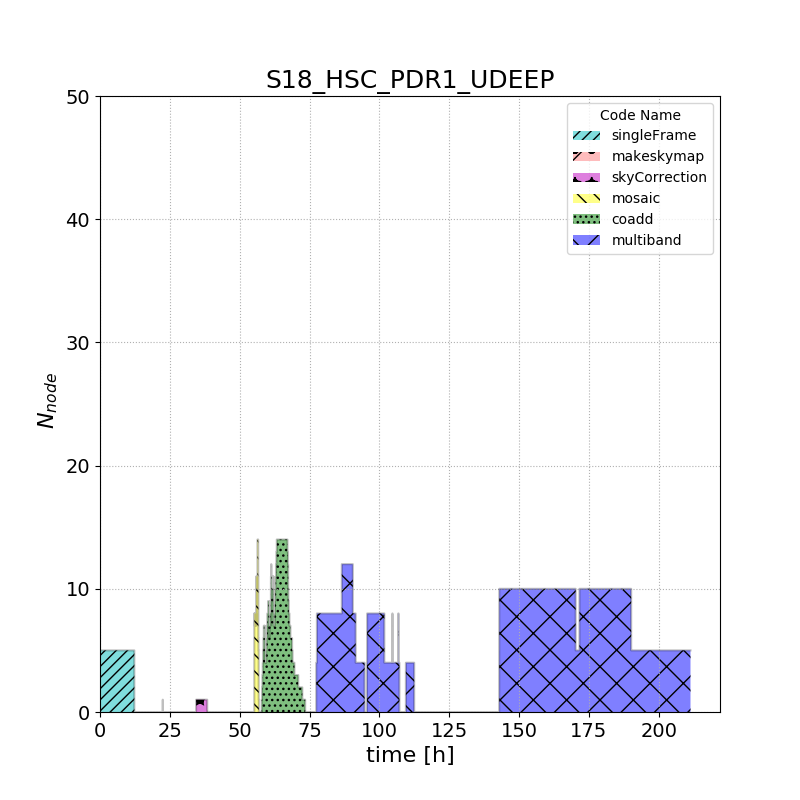
\includegraphics[width=0.50\textwidth]{usage-S18_HSC_PDR1_UDEEP.png}
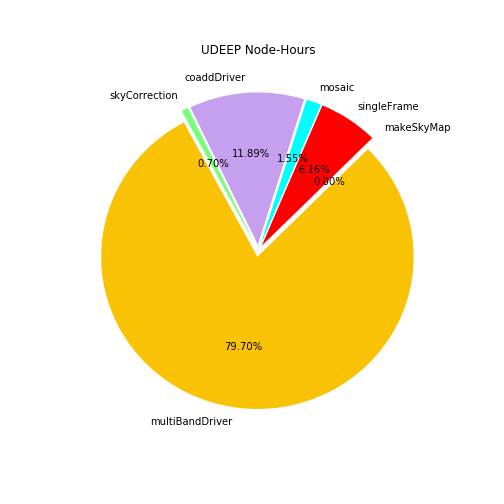
\includegraphics[width=0.50\textwidth]{PDR1_UDEEP_pie.png}
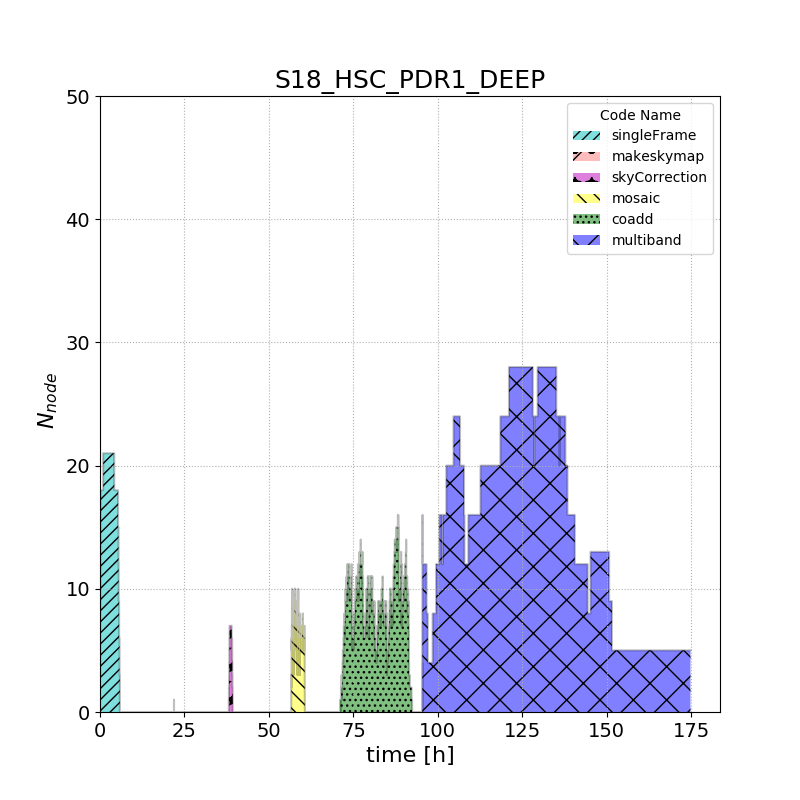
\includegraphics[width=0.50\textwidth]{usage-S18_HSC_PDR1_DEEP.png}
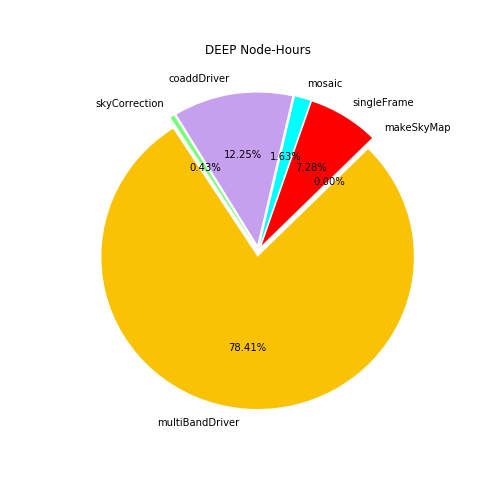
\includegraphics[width=0.50\textwidth]{PDR1_DEEP_pie.png}
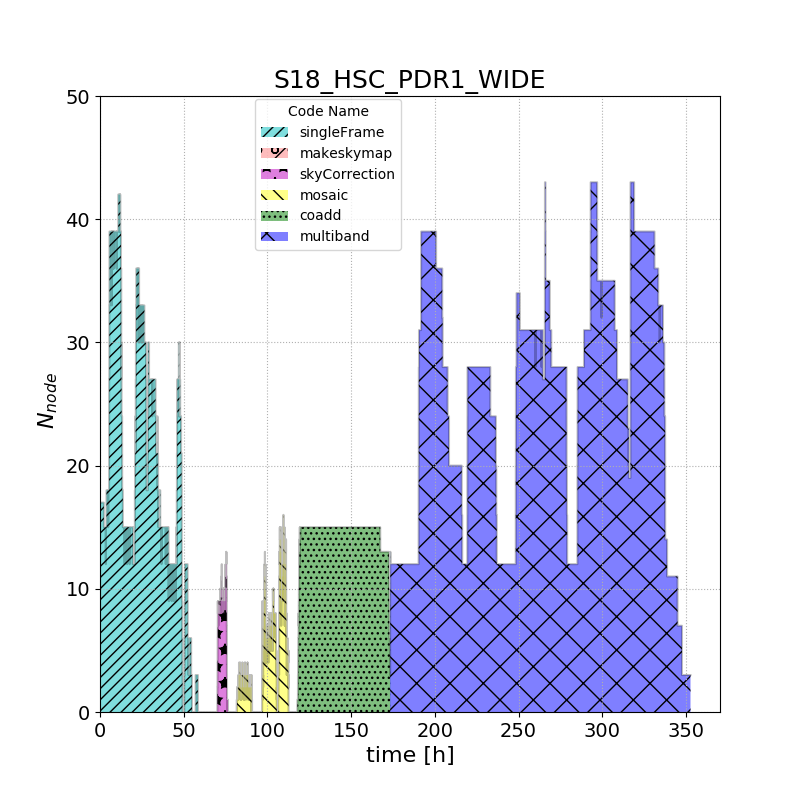
\includegraphics[width=0.50\textwidth]{usage-S18_HSC_PDR1_WIDE.png}
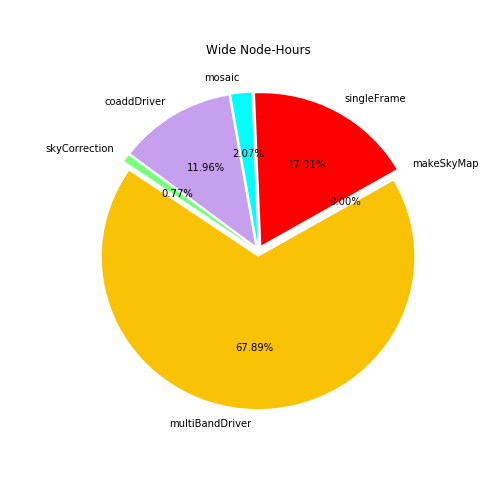
\includegraphics[width=0.50\textwidth]{PDR1_Wide_pie.png}
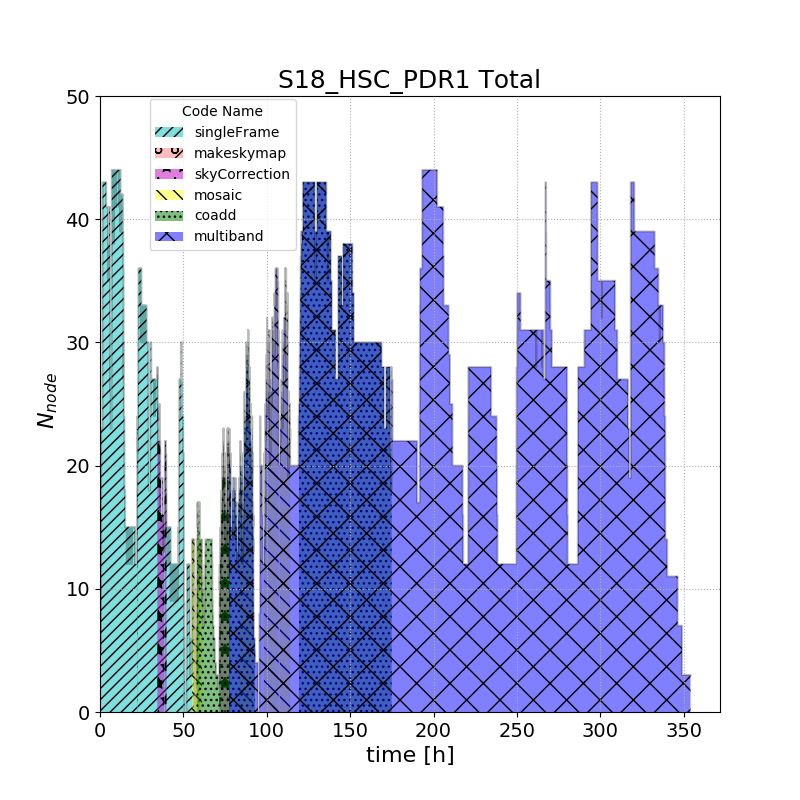
\includegraphics[width=0.50\textwidth]{usage-S18_HSC_PDR1_Total.png}
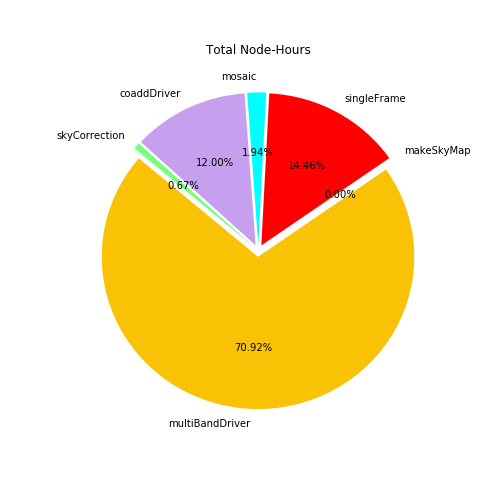
\includegraphics[width=0.50\textwidth]{PDR1_Total_pie.png}
\caption{Node-hours usage from Slurm accounting}
\label{figs}
\end{figure}


\section{Low-level processing details}
This section includes low-level details that may only be of interest to the operation team.

The first singleFrame job that contributed to the output data products started on April 20, the last multiband job finished on May 5.

In the beginning we attempted to run each visit as its own singleFrameDriver. One advantage of doing so is that each visit would have its own log file. During the attempt, many jobs took much longer than expected and timed out. The IO wait time on GPFS was excessively high (e.g. \approx5 sec), likely because too many nodes simultaneously put locks on the same folders and sometimes same files. So we changed the strategy, and grouped multiple visits into fewer singleFrameDriver calls. The modified strategy was then to group all UDEEP visits into one singleFrameDriver job, DEEP visits into 7 jobs, and WIDE visits into 149 jobs.

Each of the grouped singleFrameDriver used multiple nodes. A non-small percentage (~30\%) of jobs failed at slurm failing to launch the job. This is after singleFrameDriver.py successfully submitted the job to slurm, the job waited in the queue for its turn, and the job started trying once it got its turn, but then the job failed to launch with a message about socket timeout. This failure wasn't restricted to one specific worker node. 
\jira{DM-14181} was filed for further investigations. All failures were resubmitted iteratively, with many failed again in the iterations, and eventually were all pushed though.  On Apr 24 morning, the verification cluster used a brief downtime and the LDAP timeout in sssd.conf was increased on verify nodes. Afterwards the socket timeout problems were no longer seen.

The execution of skyCorrection.py is independent per visit. The visit grouping of singleFrameDriver was used, resulting in 157 slurm jobs.

A sqlite3 file was made for each layer to store information of what tract/patch overlaps what ccds, checking through each calexp using skymap.findTractPatchList  and geom.convexHull features. Different from the S17B HSC PDR1 reprocessing, only tracts that are in the PDR1 were included this time; the tract IDs can be found in https://hsc-release.mtk.nao.ac.jp/doc/index.php/database/ (except tract=9572) or the first table on the S17B HSC PDR1 reprocessing page (\url{https://confluence.lsstcorp.org/display/DM/S17B+HSC+PDR1+reprocessing}).  A few additional tracts were processed in the first place but were manually cleaned up afterwards.

mosaic.py and coaddDriver.py were run for each tract x filter combination, using all visits overlapping that tract in that filter for each layer, i.e. 69 jobs in UDEEP, 218 jobs in DEEP, and 455 jobs in WIDE. 1 node was used for each job.

multiBandDriver.py was then run for each tract.  There are 11 tracts in total in the UDEEP layer, so the starting plan was to run multiband in 11 jobs. In the first attempt, each used 4 nodes and 12 cores per node. Some jobs failed to launch due to \jira{DM-14181}, before the sssd timeout window was updated on Apr 24 morning. Those jobs were resubmitted.   Some jobs failed because they went out of memory; they were tract=8523 and tract=9813. I then attempted to run them with 5 nodes and 6 cores each (without reusing the existing data).  tract=8523finished but tract=9813 went out of memory again. I continued  tract=9813 using the --reuse-outputs-from option, and then it completed. Therefore, 12 slurm jobs in total contributed to the output data products in UDEEP.

In the DEEP layer, there are 37 tracts in total. In the first attempt, 37 slurm jobs were submitted and each used 4 nodes and 12 cores. All completed except the job of tract=9463 went out of memory and failed. tract=9463 was then re-run using 5 nodes and 6 cores each (without reusing the existing data); it competed.  In the WIDE layer, there are 91 tracts in total. It was completed in 91 slurm jobs, using either 4 or 3 nodes per job, 12 cores per node.

In many cases, we set a larger time limit or allowed more memory than strictly necessary; this was not optimal but helped minimizing manual intervention throughout the campaign, arguably improving the overall throughput.

The campaign mainly used the 15 worker nodes under the slurm reservation ( IHS-749 - Jira project doesn't exist or you don't have permission to view it. ) but also used other workers outside of the reservation if they were idle.  Throughout the campaign, we did not occupy the entire cluster and at least some worker nodes in the normal queue were available for or used by other users. The intention was to allow developers to bypass the production jobs for their small jobs (a few nodes) and in a short queue for large jobs. This balance was kept manually.  It would be nice to have a production queue doing this for me (and also have a more consistent balance).
